\begin{figure}[h]
    \centering
    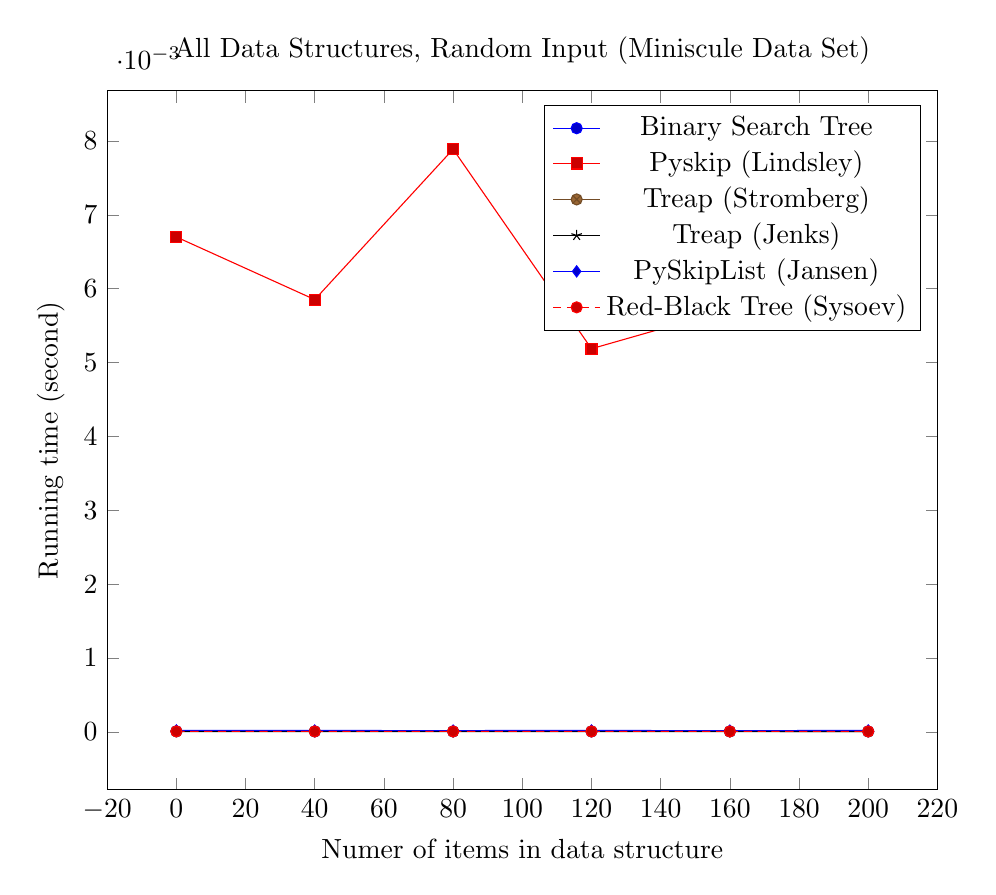
\begin{tikzpicture}
        \begin{axis}[
            xlabel={Numer of items in data structure},
            ylabel={Running time (second)},
            title={All Data Structures, Random Input (Miniscule Data Set)},
            width=\textwidth
        ]
		\addplot coordinates {
			(0, 7.499265885080319e-06)
			(40, 5.119980724810347e-06)
			(80, 5.089863191098942e-06)
			(120, 5.119980724810347e-06)
			(160, 5.300685926812321e-06)
			(200, 5.059745657431947e-06)
		};
		\addplot coordinates {
			(0, 0.006699434543305261)
			(40, 0.005851746440484007)
			(80, 0.007888053127329365)
			(120, 0.00518651035666684)
			(160, 0.005721969987877706)
			(200, 0.006835595913050696)
		};
		\addplot coordinates {
			(0, 5.330803460523726e-06)
			(40, 6.0536242687092566e-06)
			(80, 4.939275522719555e-06)
			(120, 6.143976869754653e-06)
			(160, 5.119980724721529e-06)
			(200, 4.517630051292798e-06)
		};
		\addplot coordinates {
			(0, 2.8009306317855477e-06)
			(40, 2.319050093024799e-06)
			(80, 2.1383448909340075e-06)
			(120, 2.288932559313395e-06)
			(160, 2.108227357222603e-06)
			(200, 2.1383448910228252e-06)
		};
		\addplot coordinates {
			(0, 1.9124633883738083e-05)
			(40, 1.716699419489487e-05)
			(80, 1.6805583790713287e-05)
			(120, 1.761875719994421e-05)
			(160, 1.617311558357315e-05)
			(200, 1.7859697469368996e-05)
		};
		\addplot coordinates {
			(0, 6.324682071756626e-06)
			(40, 5.2404508594783294e-06)
			(80, 5.150098258432933e-06)
			(120, 5.180215792144338e-06)
			(160, 5.180215792144338e-06)
			(200, 5.270568393189734e-06)
		};
        \legend{Binary Search Tree, Pyskip (Lindsley), Treap (Stromberg), Treap (Jenks), PySkipList (Jansen), Red-Black Tree (Sysoev)}
        \end{axis}
    \end{tikzpicture}
    \caption{Average of 10 operations, benchmarked every 40, starting at 0.}
\end{figure}